%%%%%%%%%%%%%%%%%%%%%%%%%%%%%%%%%%%%%%%%%
% Thin Sectioned Essay
% LaTeX Template
% Version 1.0 (3/8/13)
%
% This template has been downloaded from:
% http://www.LaTeXTemplates.com
%
% Original Author:
% Nicolas Diaz (nsdiaz@uc.cl) with extensive modifications by:
% Vel (vel@latextemplates.com)
%
% License:
% CC BY-NC-SA 3.0 (http://creativecommons.org/licenses/by-nc-sa/3.0/)
%
%%%%%%%%%%%%%%%%%%%%%%%%%%%%%%%%%%%%%%%%%

%----------------------------------------------------------------------------------------
%	PACKAGES AND OTHER DOCUMENT CONFIGURATIONS
%----------------------------------------------------------------------------------------

\documentclass[a4paper, 11pt]{article} % Font size (can be 10pt, 11pt or 12pt) and paper size (remove a4paper for US letter paper)

\usepackage[protrusion=true,expansion=true]{microtype} % Better typography
\usepackage{graphicx} % Required for including pictures
\usepackage{wrapfig} % Allows in-line images
%\usepackage{indentfirst} % indentent in the first sentence of each para
\usepackage{mathpazo} % Use the Palatino font
\usepackage[T1]{fontenc} % Required for accented characters
\usepackage{amsmath} \usepackage{amssymb} %>= <=
\usepackage{hyperref}\usepackage{url} % for refernce including website 
\linespread{1.05} % Change line spacing here, Palatino benefits from a slight increase by default

\makeatletter
\renewcommand\@biblabel[1]{\textbf{#1.}} % Change the square brackets for each bibliography item from '[1]' to '1.'
\renewcommand{\@listI}{\itemsep=0pt} % Reduce the space between items in the itemize and enumerate environments and the bibliography

\renewcommand{\maketitle}{ % Customize the title - do not edit title and author name here, see the TITLE block below
\begin{flushright} % Right align
{\LARGE\@title} % Increase the font size of the title

\vspace{50pt} % Some vertical space between the title and author name

{\large\@author} % Author name
\\\@date % Date

\vspace{40pt} % Some vertical space between the author block and abstract
\end{flushright}
}

%----------------------------------------------------------------------------------------
%	TITLE
%----------------------------------------------------------------------------------------

\title{\textbf{Citi Bike Ridership Mini-Research:}\\ % Title
{Young People Are More Likely to Use Citi Bikes on Weekends} }% Subtitle

\author{\textsc{Ziman Zhou, Dongjie Fan} % Author
\\{\textit{New York University, Center for Urban Science and Progress(CUSP)}}} % Institution

\date{\today} % Date
%----------------------------------------------------------------------------------------

\begin{document}

\maketitle % Print the title section

%----------------------------------------------------------------------------------------
%	ABSTRACT AND KEYWORDS
%----------------------------------------------------------------------------------------

%\renewcommand{\abstractname}{Summary} % Uncomment to change the name of the abstract to something else

\begin{abstract}
This study aims to find out whether or not young people ride bikes on weekends more often than that of middle-aged people. The analysis performs a hypothesis test (Z-test) to compare the ratio of the number of young people using citi bikes on weekends over weekdays to that of mid-age people. The result shows that the under 5\% significance level, the ratio of the number of young people biking on weekends over week days (7 days) is greater than the counterpart of middle-aged people.
\end{abstract}

\hspace*{3,6mm}\textit{Keywords:} Citi Bike, Hypothesis Test, Z-test , Age % Keywords

\vspace{30pt} % Some vertical space between the abstract and first section

%----------------------------------------------------------------------------------------
%	ESSAY BODY
%----------------------------------------------------------------------------------------

\section*{Introduction}
%\setlength{\parindent}{2em}

In a fast pace modern city like New York, citi bike has become not only one of the most popular alternatives for commuting, but also a crucial component of a city's gradually formed network system of both transportation and social activities. As a source from which quite comprehensive datasets can be acquired, citi bike is a great subject for researchers to study citizen's behavior through patterns in its ridership. This study aims to find out whether or not young people ride bikes on weekends more often than that of middle-age people, with the assumption that the bikers' usage of citi bikes fully reflects their personal preferences --- biking only for general use rather than heavily commuting purpose. 

%------------------------------------------------

\section*{Data Availability and Processing}
\setlength{\parindent}{0pt}
%\setlength{\parindent}{2em}
All processed data used to perform the statistical test is from:

$https://s3.amazonaws.com/tripdata$ which is documented on a monthly basis. The data wrangling process follows the idea of reproducibility and includes the following stages:
\begin{enumerate}
\item Enable checking and downloading data to a pointed directory each time when searching for data of a specific month, so the existed data becomes retrievable. We choose \textbf{February 2015} citi bike data for our research.
\item Read the data with Pandas Dataframe; select and modify the attributes as needed(i.e. create a binary "age group" by calculating the ages using "birth year"). Label each row with $ 18 \leqslant age < 40$ and $ 40 \leqslant age < 60$ as \textbf{young} and \textbf{middle-aged} respectively.
\item Plots histograms to visualize the normalized fraction of young and middle-aged bikers' average biking trip counts as well as each individual group on each day of the week.
\item Considers the errors of average daily riding counts on weekdays and weekends for both biker groups.
\end{enumerate}

% 1.Enable checking and downloading data to a pointed directory each time when searching for data of a specific month, so the existed data becomes retrievable. We choose \textbf{February 2015} citi bike data for our research.

% 2.Read the data with Pandas Dataframe; select and modify the attributes as needed(i.e. create a binary "age group" by calculating the ages using "birth year"). Label each row with $ 18 \leqslant age < 40$ and $ 40 \leqslant age < 60$ as \textbf{young} and \textbf{middle-aged} respectively.

% 3.Plots histograms to visualize the normalized fraction of young and middle-aged bikers' average biking trip counts as well as each individual group on each day of the week.
% \begin{wrapfigure}{l}{0.8\textwidth} % Inline image example
% \begin{center}
% 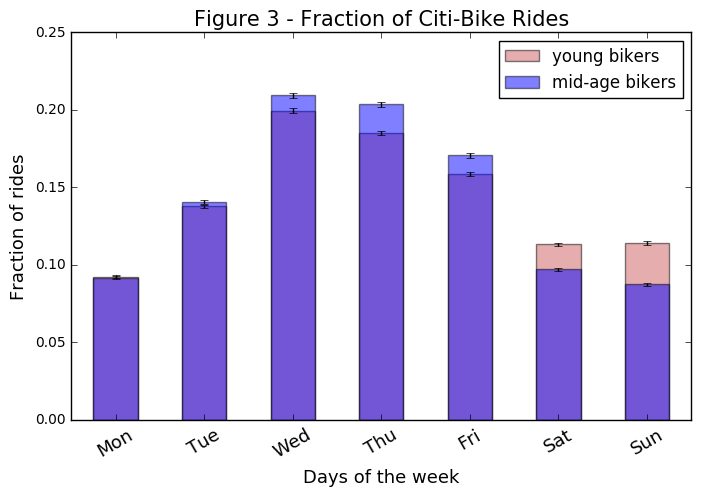
\includegraphics[width=0.8\textwidth]{image.png}
% \end{center}
% \caption{citi bike}
% \end{wrapfigure}
% 4.Consider the errors of average daily riding counts on weekdays and weekends for both biker groups.

%{\centering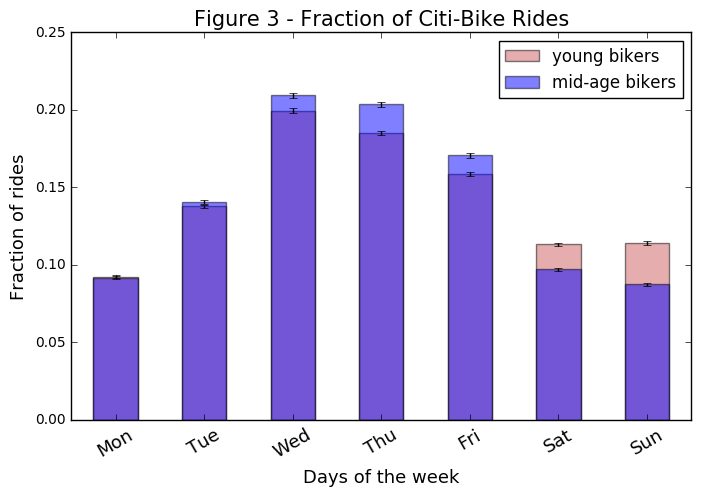
\includegraphics[width=12cm]{image.png}

\begin{figure}[h]
\centering
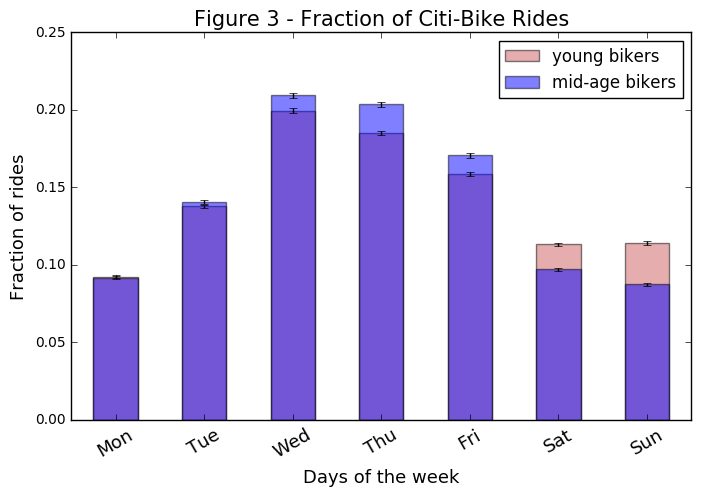
\includegraphics[width = 11.5cm ]{image.png}
\end{figure}

%------------------------------------------------


\section*{Analysis}
Since the number of population is large (>30) and the standard deviation of population is known, we choose Z-test to do hypothesis test\cite{Z-testvsT-test2}\cite{Z-testvsT-test}. According to the question we focus on, we set 
$$ H_{0}:  \frac{\# \,of\,young\, on\, weekends}{\#\,of\,young\, on \,week \,days} \leqslant \frac{\# \,of\,middle-aged\, on\, weekends}{\#\,of\,middle-aged\, on \,week \,days}$$
$$ H_{a}:  \frac{\# \,of\,young\, on\, weekends}{\#\,of\,young\, on \,week \,days} \ > \frac{\# \,of\,middle-aged\, on\, weekends}{\#\,of\,middle-aged\, on \,week \,days}$$

According to the formula\cite{ProportionZTest}, we can get $z-score = 24.4665$ and corresponding p value is lower than 0.05. Thus we choose to reject $H_{0}$, and choose $H_{a}$ which is the ratio of the number of young people biking on weekends over week days (7 days) is greater than the counterpart of middle-aged people.

\section*{Conclusion}
Based on the result of Z-test, we can conclude that under the 0.05 statistical significance, young riders is much more likely to ride citibike than middele-aged people. The reasons behind the result might be diverse, for example, there are more social activities on weekends for young people which make them ride citi bike much more. Furthur research might foucs on extracting data from different months in avoid of seasonal influence.
%And furthur researched might foucs on whether there is any difference between male and female young riders using citi bike on weekends.
%----------------------------------------------------------------------------------------
%	BIBLIOGRAPHY
%----------------------------------------------------------------------------------------

\bibliographystyle{unsrt}

\bibliography{sample}

%----------------------------------------------------------------------------------------

\end{document}